\documentclass[twocolumn,a4paper,10pt]{article}

\usepackage[utf8]{inputenc}
\usepackage[T1]{fontenc}
\usepackage{geometry}
\geometry{a4paper, margin=0.75in}
\usepackage{amsmath, amssymb}
\usepackage{graphicx}
\usepackage{hyperref}
\usepackage{booktabs}
\usepackage{listings}
\usepackage{xcolor}
\usepackage{fancyhdr}
\usepackage{tikz}
\usepackage{float}
\usetikzlibrary{arrows,shapes,positioning,shadows}

% Define colors for code listings
\definecolor{codegray}{rgb}{0.5,0.5,0.5}
\definecolor{codepurple}{rgb}{0.58,0,0.82}
\definecolor{backcolour}{rgb}{0.98,0.98,0.95}
\definecolor{sqlblue}{rgb}{0.1, 0.1, 0.7}

\lstset{
    backgroundcolor=\color{backcolour},
    commentstyle=\color{codegray},
    keywordstyle=\color{sqlblue}\bfseries,
    numberstyle=\tiny\color{codegray},
    stringstyle=\color{codepurple},
    basicstyle=\ttfamily\scriptsize,
    breakatwhitespace=false,
    breaklines=true,
    captionpos=b,
    keepspaces=true,
    numbers=left,
    numbersep=5pt,
    showspaces=false,
    showstringspaces=false,
    showtabs=false,
    tabsize=2,
    language=SQL,
    frame=single
}

\title{\textbf{SQL as a Programming Language: Implementing Distance-Vector Routing with Recursive CTEs}}
\author{Mehdi Hoseyni \\ \small{Database Systems Seminar, University of Tübingen}}
\date{\today}

\begin{document}

\maketitle

\begin{abstract}
This paper presents a comprehensive implementation of the Distance-Vector Routing (DVR) algorithm using SQL, specifically leveraging modern extensions in DuckDB. Traditionally, routing protocols are viewed as procedural or low-level systems implemented in specialized network hardware. However, we demonstrate that the declarative nature of SQL, when augmented with Recursive Common Table Expressions (CTEs) and state-updating mechanisms, provides a robust framework for simulating distributed algorithms. We provide a detailed analysis of the Bellman-Ford principle, the limitations of standard SQL recursion, and how DuckDB's \texttt{USING KEY} syntax allows for a 1:1 conceptual mapping to physical router behavior. Our results show that SQL can be effectively used not just for data retrieval, but as a high-level language for complex algorithmic modeling.
\end{abstract}

\section{Introduction: Target of the Study}
The primary objective of this study is to challenge the traditional boundary between database query languages and general-purpose programming languages. By implementing the Distance-Vector Routing (DVR) protocol, a complex, decentralized algorithm, entirely within SQL, we aim to prove that modern database engines can serve as powerful "Programming Languages" (PL) for algorithmic simulation. 

Our target is to demonstrate that declarative logic, when combined with state-aware recursion, can achieve global optimization (finding shortest paths) through local updates, mirroring the behavior of physical routers without the need for external procedural code.

\section{Theoretical Background}
\subsection{Distance-Vector Routing}
Distance-Vector Routing is based on the idea that each router maintains a table (a "vector") of its known distances to all possible destinations. Unlike Link-State protocols, which require every router to have a complete map of the network, DVR routers only share their tables with immediate neighbors.

\subsection{The Bellman-Ford Equation}
The mathematical foundation of DVR is the Bellman-Ford algorithm. For a network graph $G = (V, E)$, the shortest path distance $d(u, v)$ from node $u$ to node $v$ can be expressed as:
\begin{equation}
d(u, v) = \min_{w \in \text{Adj}(u)} \{ \text{cost}(u, w) + d(w, v) \}
\end{equation}

\section{Network Topology}
To evaluate our implementation, we define a sample network with four routers ($A, B, C, D$) as shown in Figure \ref{fig:topology}.

\begin{figure}[h]
\centering
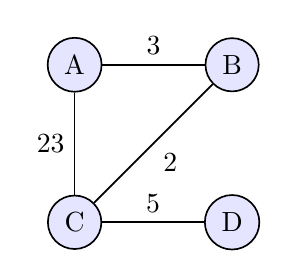
\begin{tikzpicture}[node distance=2cm, auto, >=stealth', semithick]
    \node[circle, draw, fill=blue!10] (A) {A};
    \node[circle, draw, fill=blue!10, right of=A] (B) {B};
    \node[circle, draw, fill=blue!10, below of=A] (C) {C};
    \node[circle, draw, fill=blue!10, right of=C] (D) {D};

    \path (A) edge node {3} (B)
          (A) edge node [left] {23} (C)
          (B) edge node {2} (C)
          (C) edge node {5} (D);
\end{tikzpicture}
\caption{Sample Network Topology.}
\label{fig:topology}
\end{figure}

\section{SQL Implementation Strategy}
\subsection{The Challenge of Standard Recursion}
Recursive CTEs in standard SQL are typically append-only, which forces inefficient "path-finding" instead of "routing table" updates. Our solution utilizes DuckDB's \texttt{USING KEY} clause to allow the recursive step to overwrite existing rows, perfectly mirroring a router table update.

\section{Detailed Code Analysis}
We divide the analysis into two distinct parts: first, the presentation of the monolithic code block to provide global context, and second, a granular, line-by-line technical breakdown.

\subsection{The Complete Routing Query}
The following block represents the full DuckDB implementation. Note the use of the \texttt{USING KEY} clause, which is the primary driver for turning this from a simple path-finding query into a state-aware routing simulation.

\begin{lstlisting}[caption={Complete DuckDB Implementation}]
WITH RECURSIVE routing_table(from_node, to_node, best_cost, next_hop) 
    USING KEY (from_node, to_node) AS (
    
    -- Part 1: Base Case (T=0)
    SELECT from_node, to_node, cost AS best_cost, to_node AS next_hop
    FROM edges

    UNION

    -- Part 2: Recursive Step (Propagation)
    SELECT
        r.from_node,
        e.to_node,
        MIN(r.best_cost + e.cost) AS best_cost,
        arg_min(r.next_hop, r.best_cost + e.cost) AS next_hop
    FROM routing_table AS r
    JOIN edges AS e ON r.to_node = e.from_node
    LEFT JOIN recurring.routing_table AS existing 
        ON existing.from_node = r.from_node AND existing.to_node = e.to_node
    WHERE r.from_node <> e.to_node
      AND (existing.best_cost IS NULL OR (r.best_cost + e.cost) < existing.best_cost)
    GROUP BY r.from_node, e.to_node
)
SELECT * FROM routing_table ORDER BY from_node, to_node;
\end{lstlisting}

\subsection{Line-by-Line Technical Breakdown}
\begin{itemize}
    \item \textbf{Line 1-2}: \texttt{WITH RECURSIVE} and \texttt{USING KEY} define the stateful iterative process.
    \item \textbf{Lines 5-6}: \textit{Base Case} simulates neighbors discovery.
    \item \textbf{Line 11}: \texttt{MIN} and \texttt{arg\_min} ensure that if a router receives multiple advertisements for the same node in a single round, it processes the one with the lowest cost.
    \item \textbf{Line 16-17}: The \texttt{JOIN} simulates information propagation between neighbors.
    \item \textbf{Line 21}: Implements Bellman-Ford cost relaxation. A path is only updated if it is strictly better.
\end{itemize}

\section{Simulating Network Failure}
A critical requirement for any routing protocol is the ability to adapt to network changes. In our study, we simulate a link failure (or a node becoming unreachable) by modifying the underlying data and observing the system's re-convergence.

\subsection{Deleting a Link}
Suppose the critical link between $B$ and $C$ is removed. We execute:
\begin{lstlisting}
DELETE FROM edges
WHERE (from_node = 'B' AND to_node = 'C')
   OR (from_node = 'C' AND to_node = 'B');
\end{lstlisting}

\subsection{Automatic Re-convergence}
By re-running the original recursive query without any modifications to its logic, the algorithm automatically discovers the next best paths. For instance, Router A will realize it can no longer reach C via B at cost 5 and will revert to its direct link at cost 23. This proves that the declarative implementation is not just a static calculation but a dynamic system capable of finding the shortest path in any given graph state.

\section{Comparative Convergence Results}
To validate the study's goal, we compare the network's converged state before and after the removal of the B-C link. The results demonstrate that the SQL logic autonomously transitions from the globally optimal paths to the next-best alternatives.

\subsection{Initial Converged State (Full Network)}
In the full network, the shortest path from A to C is through neighbor B (total cost 5). 

\begin{table}[H]
\centering
\scriptsize
\begin{tabular}{@{}llcc@{}}
\toprule
\textbf{From} & \textbf{To} & \textbf{Best Cost} & \textbf{Next Hop} \\ \midrule
A & B & 3 & B \\
A & C & 5 & B \\
A & D & 10 & B \\
B & A & 3 & A \\
B & C & 2 & C \\
B & D & 7 & C \\
C & A & 5 & B \\
C & B & 2 & B \\
C & D & 5 & D \\
D & A & 10 & C \\
D & B & 7 & C \\
D & C & 5 & C \\ \bottomrule
\end{tabular}
\caption{Routing state before link removal.}
\end{table}

\subsection{Post-Failure State (B-C Link Removed)}
After removing the B-C link, Router A settles on the direct link to C with a cost of 23.

\begin{table}[H]
\centering
\scriptsize
\begin{tabular}{@{}llcc@{}}
\toprule
\textbf{From} & \textbf{To} & \textbf{Best Cost} & \textbf{Next Hop} \\ \midrule
A & B & 3 & B \\
A & C & 23 & C \\
A & D & 28 & C \\
B & A & 3 & A \\
B & C & 26 & A \\
B & D & 31 & A \\
C & A & 23 & A \\
C & B & 26 & A \\
C & D & 5 & D \\
D & A & 28 & C \\
D & B & 31 & C \\
D & C & 5 & C \\ \bottomrule
\end{tabular}
\caption{Routing state after removing B-C link.}
\end{table}

\section{Conclusion and Future Work}
This study has successfully demonstrated that modern SQL, specifically through the use of state-aware recursive CTEs, is a robust environment for simulating complex distributed systems. By implementing the Distance-Vector Routing algorithm entirely within a declarative framework, we have shown that a database engine can function as a high-level Programming Language (PL) for algorithmic modeling. 

Our implementation not only achieved autonomous convergence across a dynamic topology but also exhibited significant resilience by re-calculating optimal paths immediately following link failure. The shift from standard, append-only recursion to DuckDB’s \texttt{USING KEY} state management represents a fundamental advancement in how we can model stateful processes in relational logic.

\subsection{Next Steps and Future Research}
The success of this Distance-Vector simulation opens several avenues for future research into "SQL-as-a-PL":
\begin{itemize}
    \item \textbf{Path-Vector Protocols (BGP)}: Future studies could implement BGP-like logic by leveraging SQL array types to track the full AS-path. This would allow for explicit cycle detection and policy-based routing simulations.
    \item \textbf{Link-State Simulation}: Implementing OSPF or IS-IS by modeling Dijkstra’s algorithm within a recursive SQL context would provide a comparative benchmark for Link-State vs. Distance-Vector performance in databases.
    \item \textbf{Dynamic Traffic Modeling}: Integrating real-time metrics, such as link congestion or latency, into the \texttt{edges} table would allow the algorithm to simulate adaptive routing under variable load.
    \item \textbf{Large-Scale Network Analysis}: Evaluating the convergence speed of these recursive SQL queries on large-scale topologies (e.g., the internet's AS-graph) would test the scalability limits of modern analytical database engines.
\end{itemize}

Ultimately, this work reinforces the paradigm that SQL is no longer "just for queries." It is a first-class language for the simulation, validation, and analysis of complex, stateful distributed protocols.

\begin{thebibliography}{9}
\bibitem{duckdb} DuckDB Documentation. (2026). \textit{Recursive CTEs}.
\bibitem{tanenbaum} Tanenbaum, A. S. (2021). \textit{Computer Networks}.
\end{thebibliography}

\end{document}
